\include{template}

\title{Podstawy uczenia maszynowego \\ Sprawozdanie nr. 3 \\ Tak na marginesie}
\author{Jan Izydorczyk}
\date{Maj 2022}


\begin{document}

\maketitle

\section{Dane wejściowe}

Dane wejściowe zostały wygenerowane za pomocą oficjalnego narzędzia do edycji grafiki rastrowej, autorstwa wiodącej firmy technologicznej Microsoft\cite{paint}. 


\begin{figure}[H]
        \centering
        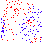
\includegraphics[width=0.6\textwidth]{img/dataimg.png}
        \caption{Obrazek bazowy}
\end{figure}

Na jego podstawie zostały wygenerowany finalny dataset.

\begin{figure}[H]
        \centering
        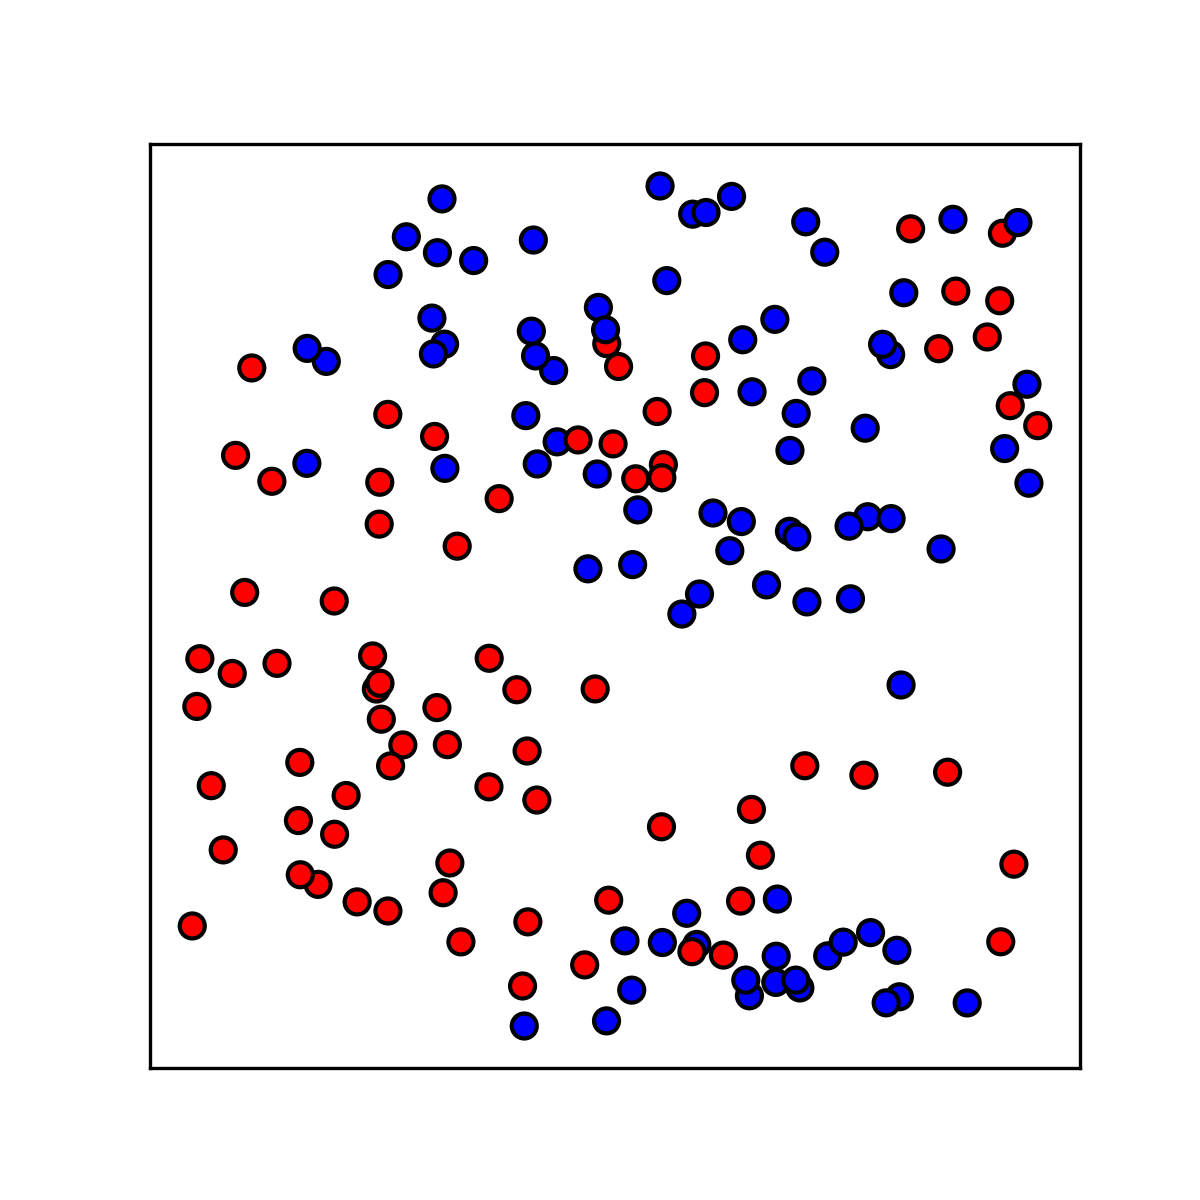
\includegraphics[width=1\textwidth]{img/pts.png}
        \caption{Finalny zbiór punktów}
\end{figure}

Punkty reprezentują dwie (prawie) liniowo separowalne klasy (nie licząc kilku wysp punktów) w przestrzeni 2D. 

\section{SVMy}

Zastosowanych zostało sześć klasyfikatorów, wszystkie oparte na SVMie:

\begin{enumerate}
    \item Liniowy SVM
    \item Oparty na pierwszym koordynacie SVM
    \item RBF SVM
    \item "Kanciasty" SVM
    \item "Prawie liniowy" SVM
    \item "Prawie cosinusowy" SVM
\end{enumerate}

\begin{figure}[H]
        \centering
        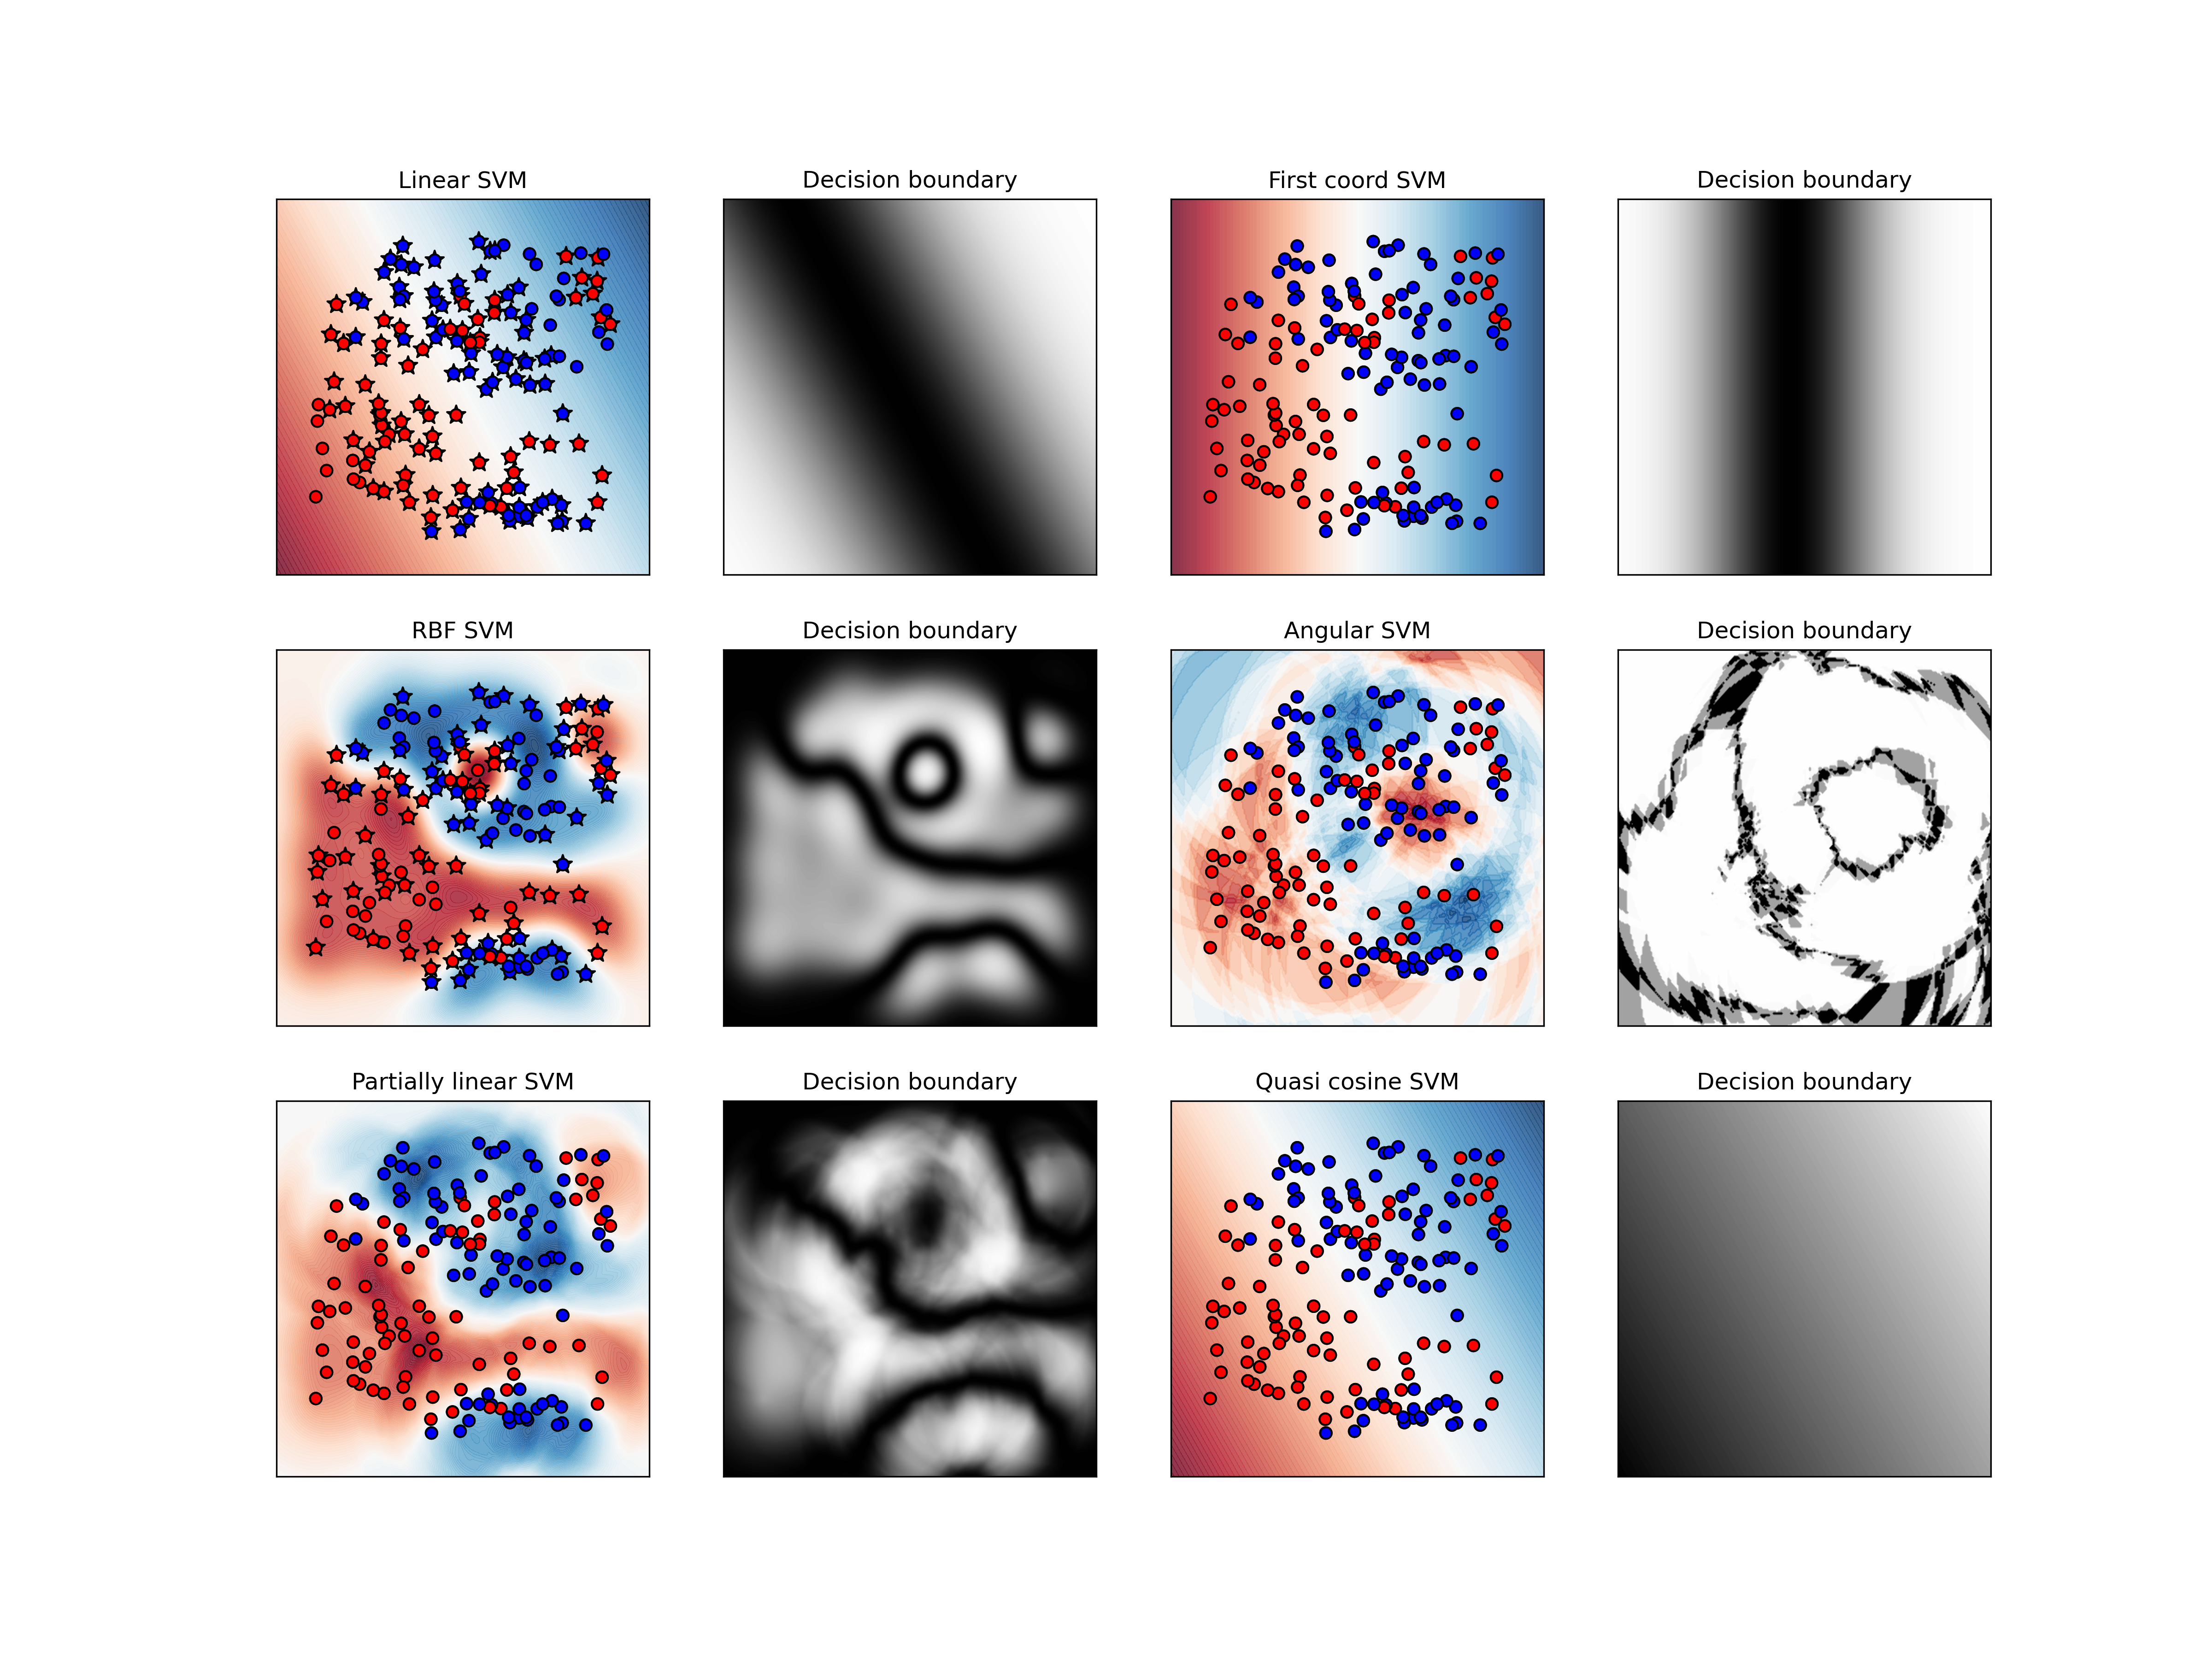
\includegraphics[width=1\textwidth]{img/all.png}
        \caption{Porównanie przykładowych rezultatów zastosowanych klasyfikatorów SVM}
\end{figure}

\subsection{Liniowy SVM}

\begin{figure}[H]
        \centering
        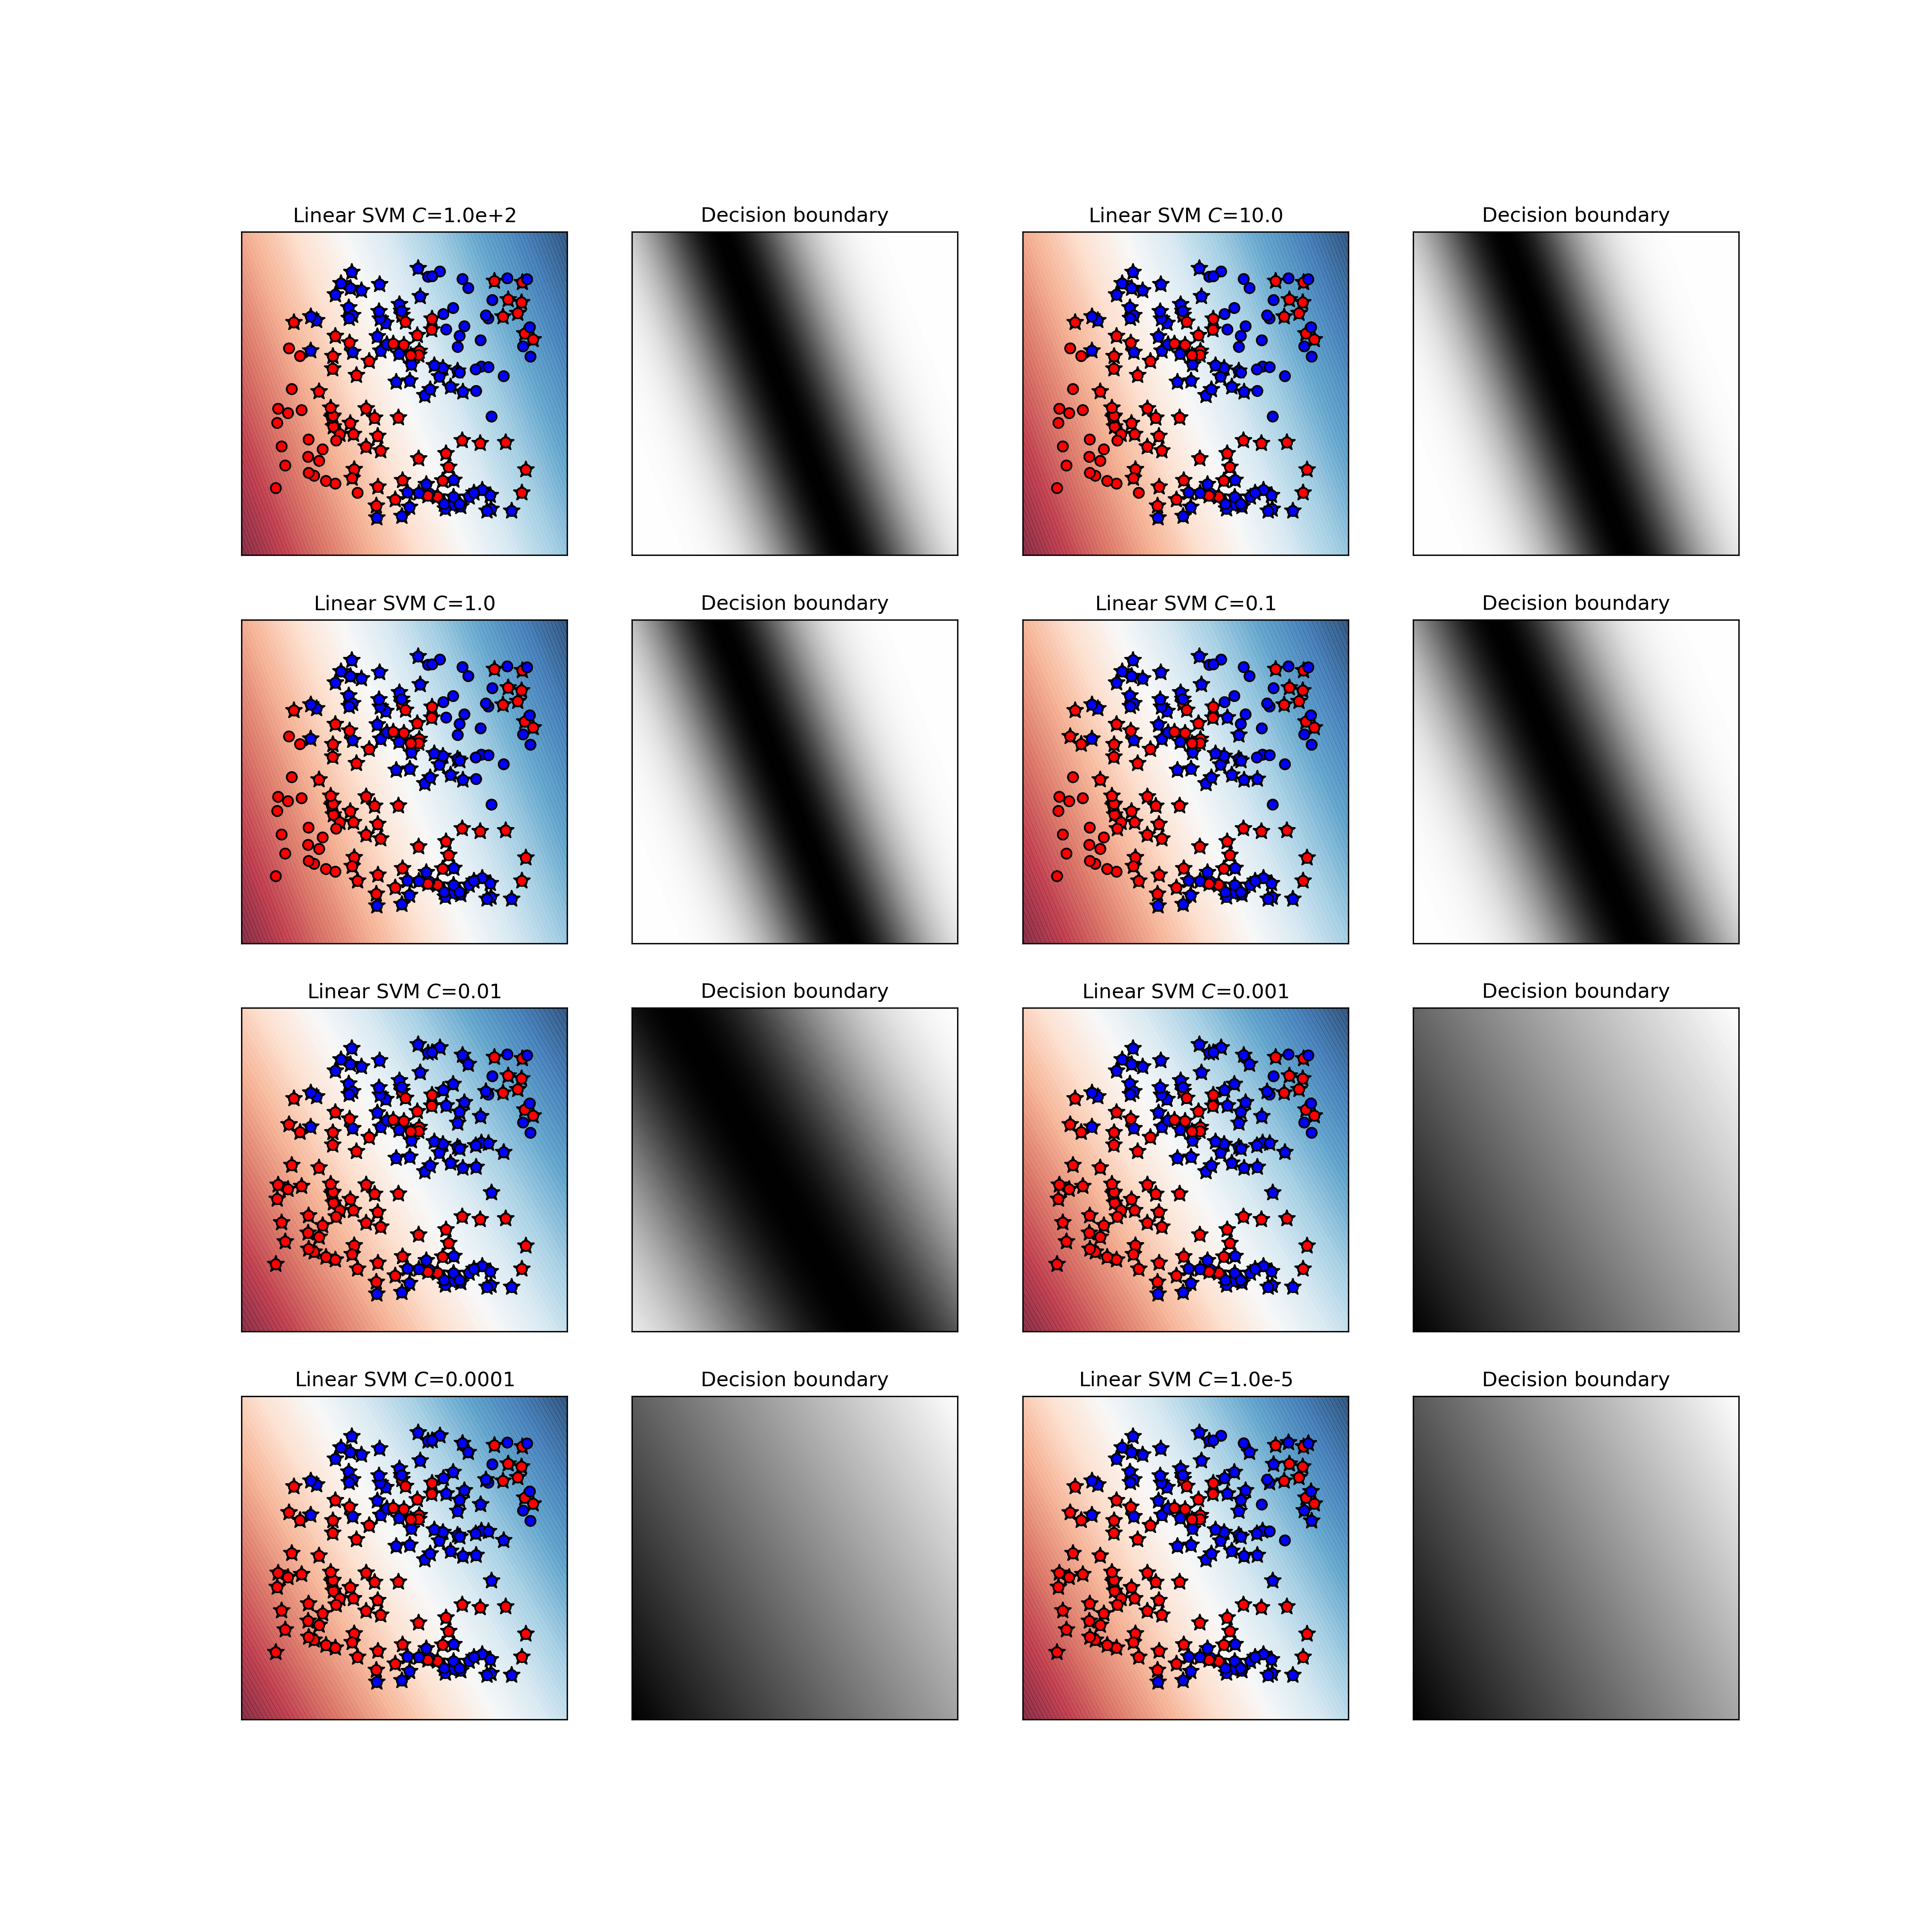
\includegraphics[width=1\textwidth]{img/lin.png}
        \caption{Liniowe SVMy\\dla różnych wartości współczynnika penalty $C$}
\end{figure}

Można zaobserwować, że dla coraz niższych wartości współczynnika kary granica decyzyjna jest coraz szersza, gdzie różnice są rzędu podwojenia szerokości. Dla wysokiego współczynnika wielkość granicy nie przekracza 30~40 procent średnicy zbioru danych.

\subsection{RBF SVM}

\begin{figure}[H]
        \centering
        \includegraphics[width=1\textwidth]{img/rbf.png}
        \caption{SVMy z kernelem $RBF$\\dla różnych wartości współczynnika $\gamma$}
\end{figure}

Dla względnie duzych wartości współczynnika $\gamma$ modele odzwierciedlaly znacznie więcej szczegółów ze zbioru danych. Dla małych wartości granice decyzyjne znacznie bardziej uogólniały obie klasy, pomijając wyspy izolowane wyspy punktów. W ogólno

\subsection{"Kanciasty" RBF SVM}

\begin{figure}[H]
        \centering
        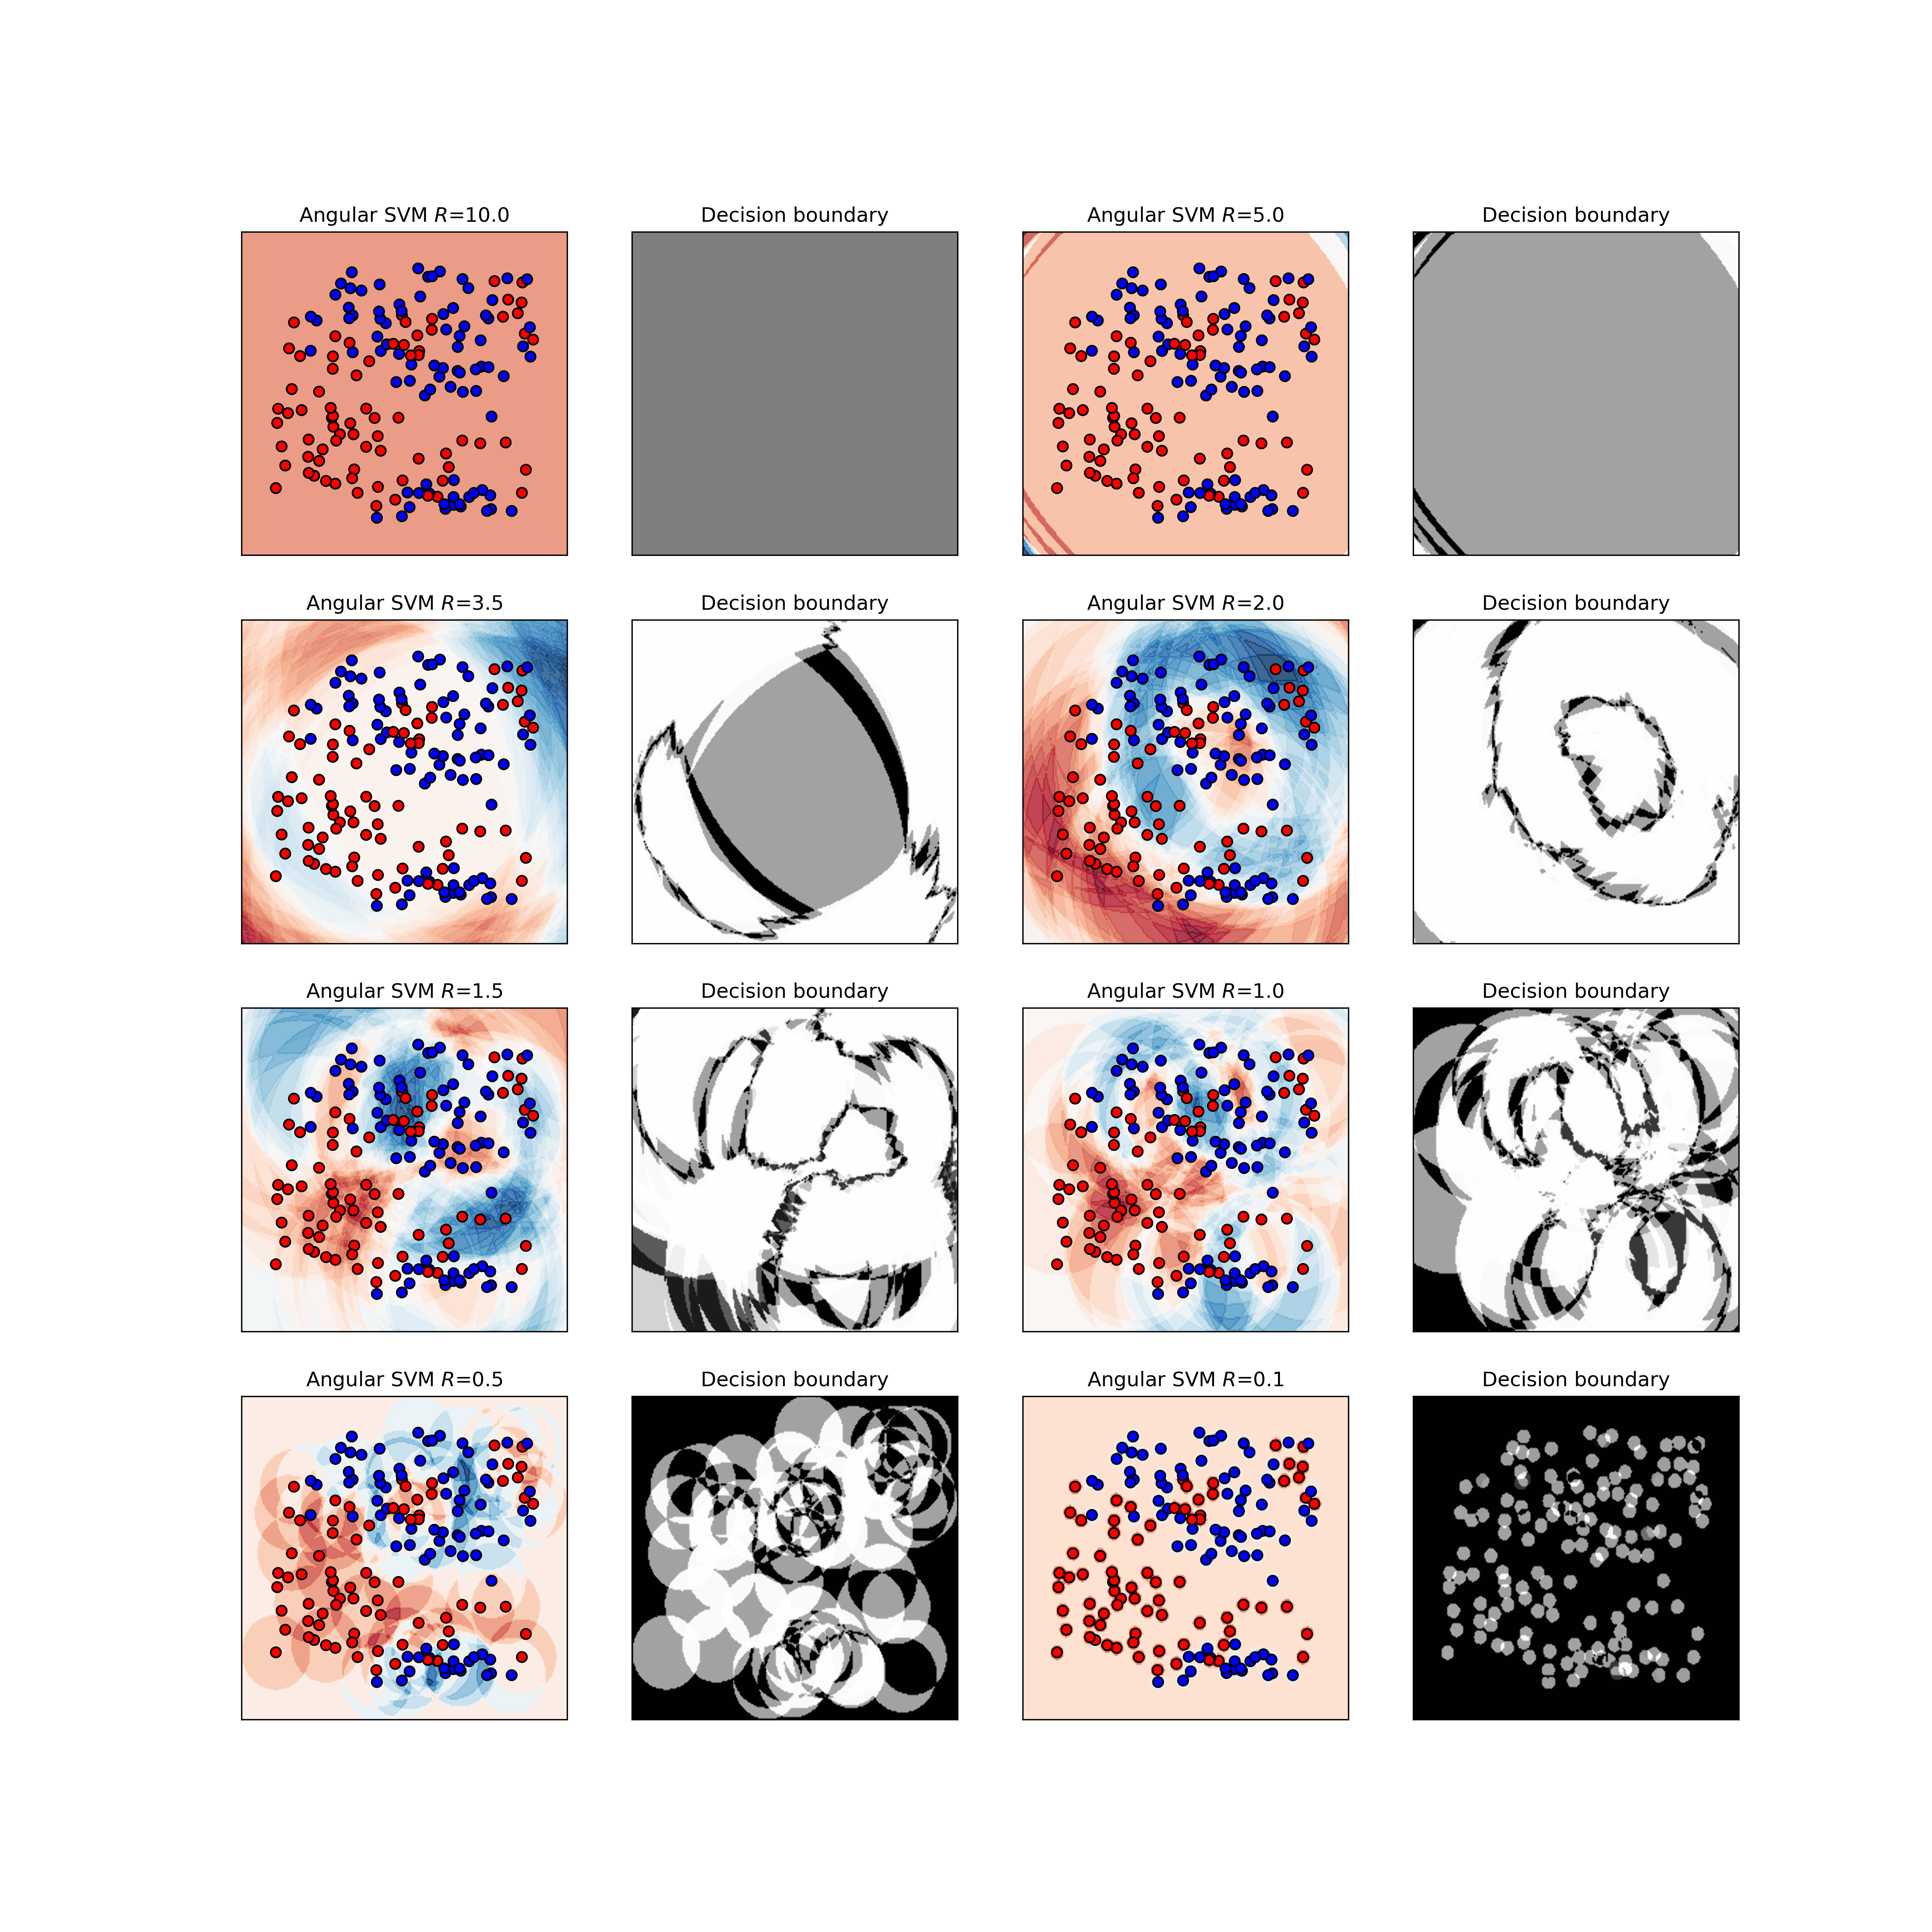
\includegraphics[width=1\textwidth]{img/kanc.png}
        \caption{SVMy z "kanciastym" kernelem $RBF$\\dla różnych wartości współczynnika promienia $R$}
\end{figure}

Rzeczywiscie jest to kanciaste jądro. Dla wartości promienia rzędu wielkości odległości punktów w data secie kernel ten zwracał sensowne wyniki, dla wartości wyzszych granice decyzyjne wydawały sie nie oddawać trendów obu klas, a dla nizszych dochodzilo do everfittingu.

\subsection{"Prawie" liniowy SVM}

\begin{figure}[H]
    \centering
    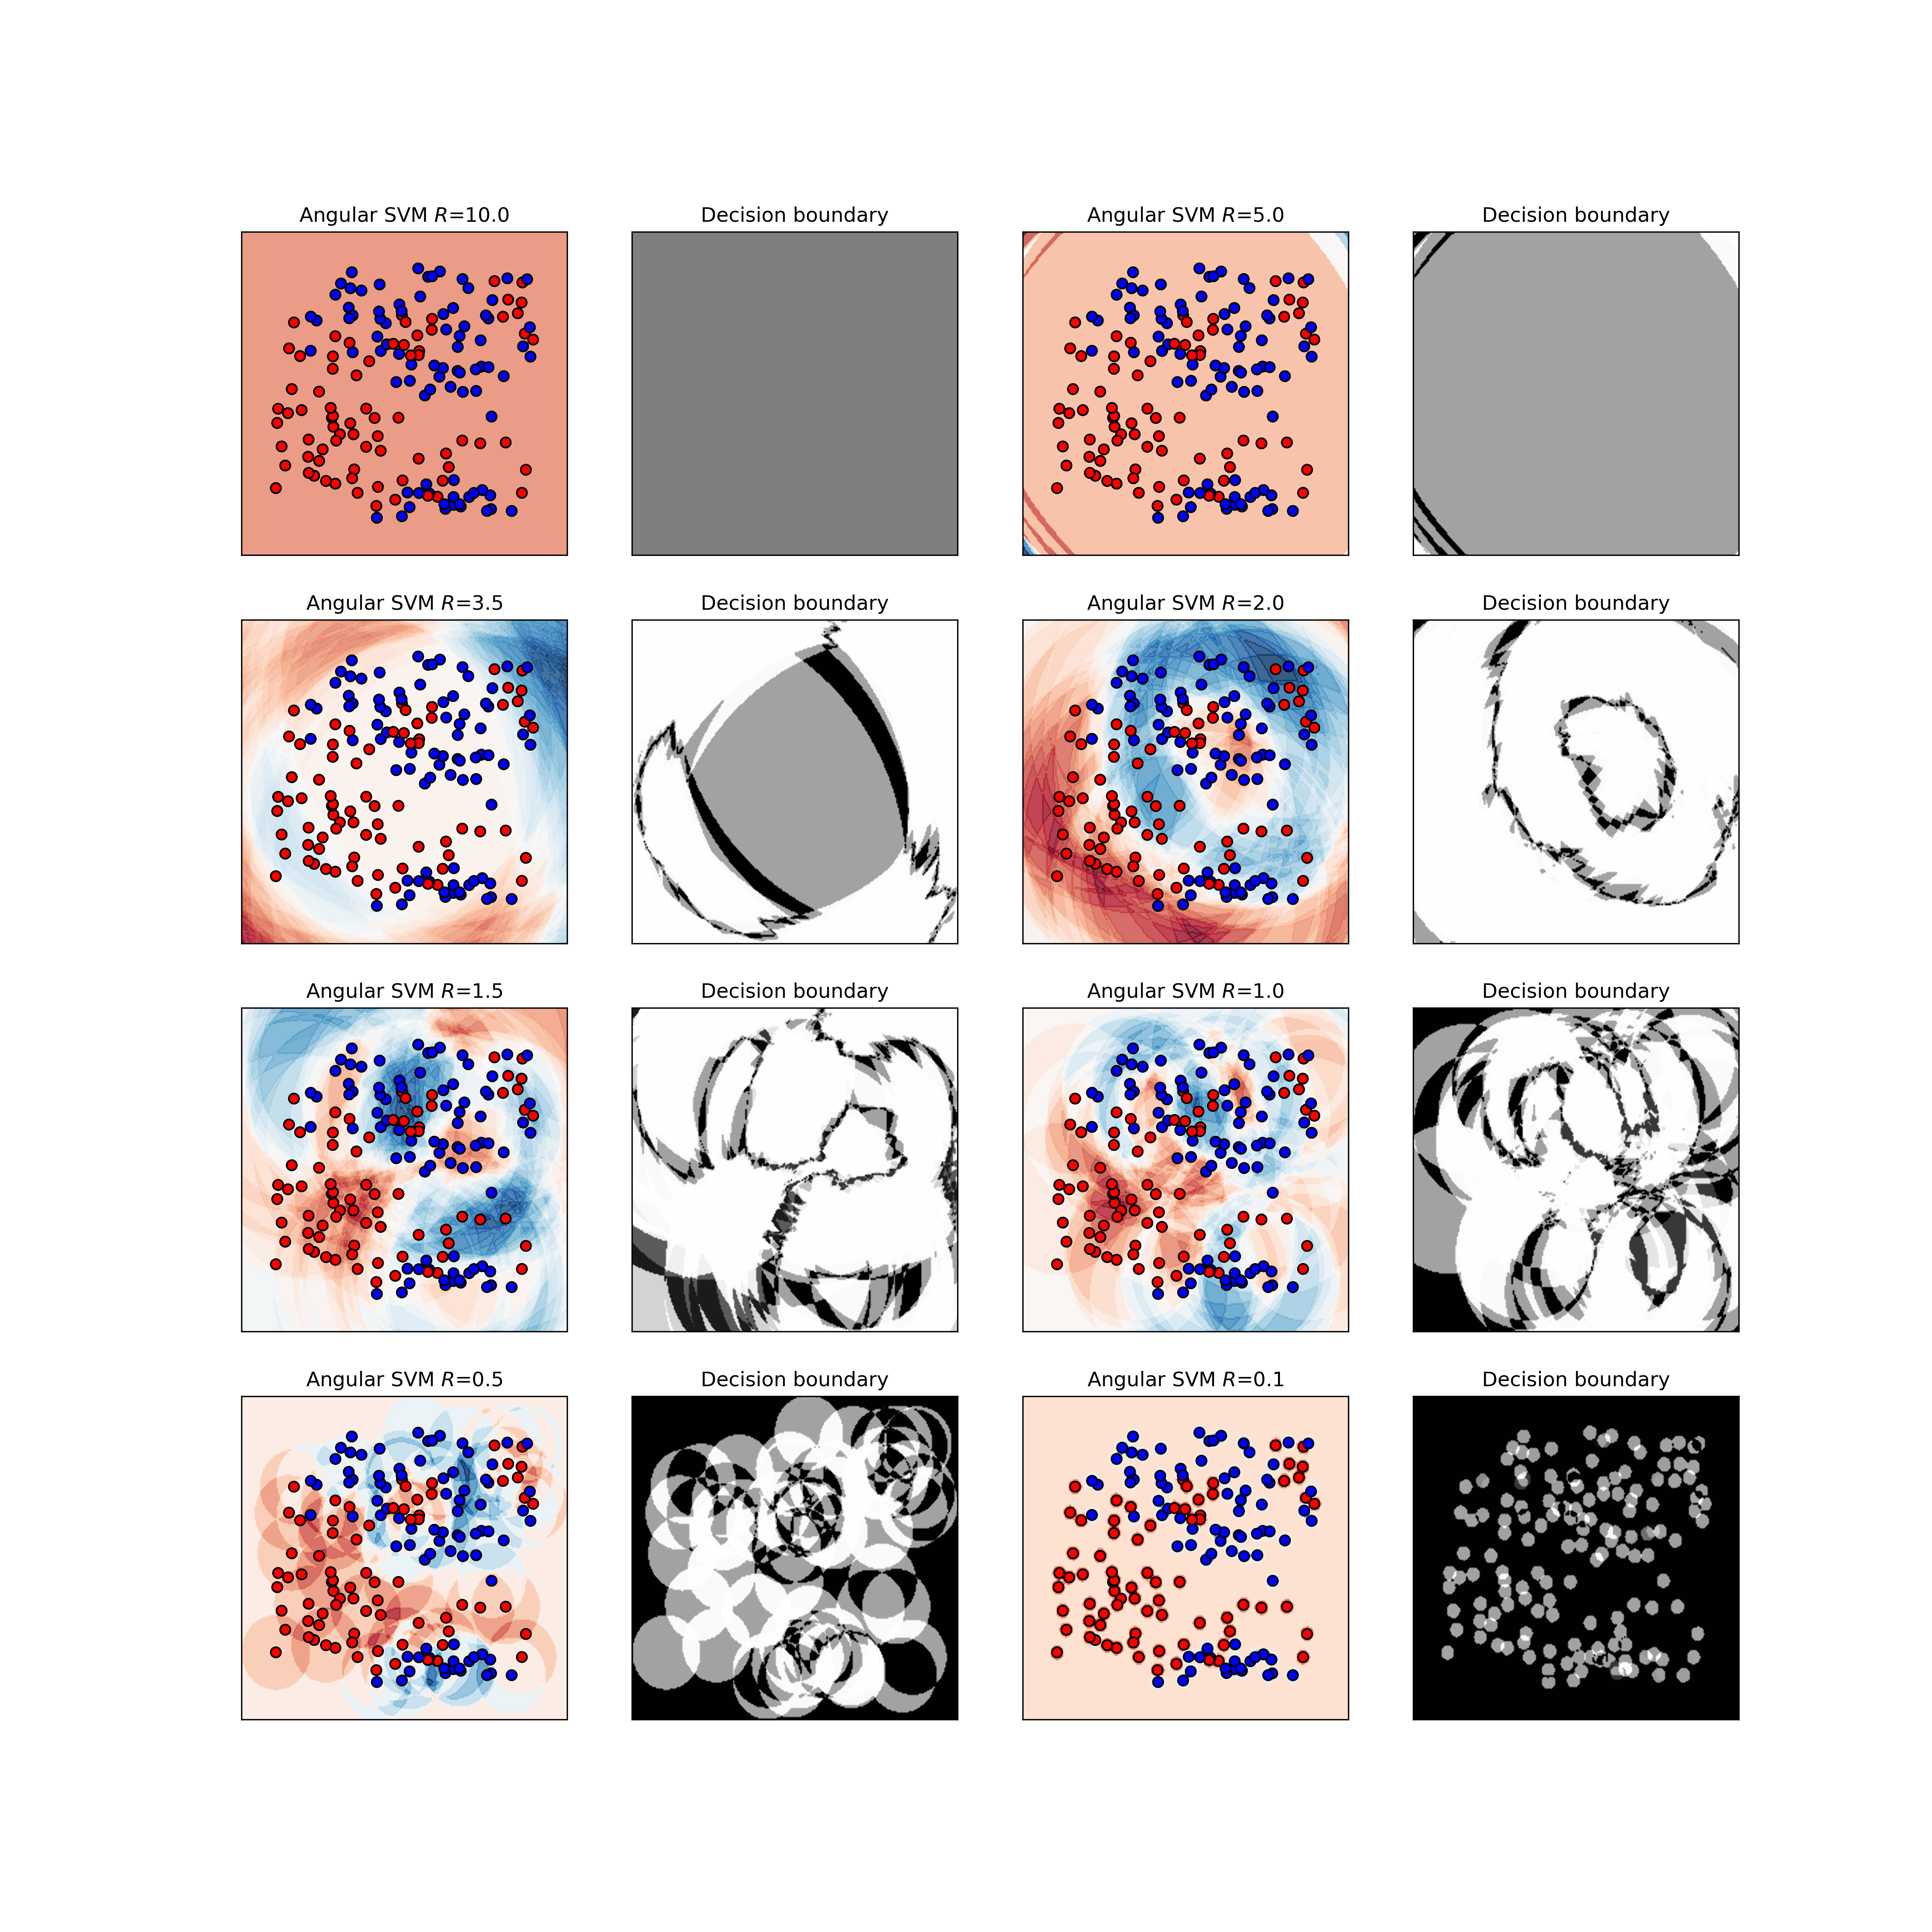
\includegraphics[width=1\textwidth]{img/kanc.png}
    \caption{SVMy z "prawie" linowym kernelem $RBF$\\dla różnych wartości współczynnika promienia $R$}
\end{figure}

Rezultaty tego jądra są podobne do 

\begin{thebibliography}{9}
    \bibitem{paint}
        Program do edycji grafiki rastrowej firmy Microsoft \\
        \url{https://apps.microsoft.com/store/detail/paint/9PCFS5B6T72H?hl=en-us&gl=US}
\end{thebibliography}

\end{document}